\section{Experimentul Rutherford. Modelul planetar al atomului}

Atomul este cea mai mică particulă a unui element care păstrează toate
caracteristicile acestuia. Din cauza dimensiunilor sale mici, nu poate fi
studiat direct, ci folosind „sonde” de mărime atomică sau subatomică.

\subsection{Experimentul Rutherford}

Fizicianul englez Ernest Rutherford a constatat că particulele alfa, emise de o
sursă radioactivă, trec printr-o foiță subțire de aur (0,1 {\textmu}m), iar
radiația {\alpha} poate fi detectată de un ecran fluorescent sub orice unghi.
Majoritatea particulelor {\alpha} sunt slab deviate; numărul particulelor deviate la
unghiuri mari este foarte mic, de o particulă din 10000.

Particulele {\alpha} sunt nuclee de heliu, având sarcina $+2e$ și masa de 7000
de ori mai mare decât a electronului. Deci particula {\alpha} poate fi deviată
numai de o particulă cu masa mare și sarcina pozitivă.

Motivul pentru care foarte puține particule sunt deviate la unghiuri mari este
concentrația sarcinei pozitive într-o regiune extrem de mică din volumul
atomului de aur.

\subsubsection*{Simularea experimentului}

\begin{wrapfigure}{r}{0.4\textwidth}
    \centering
    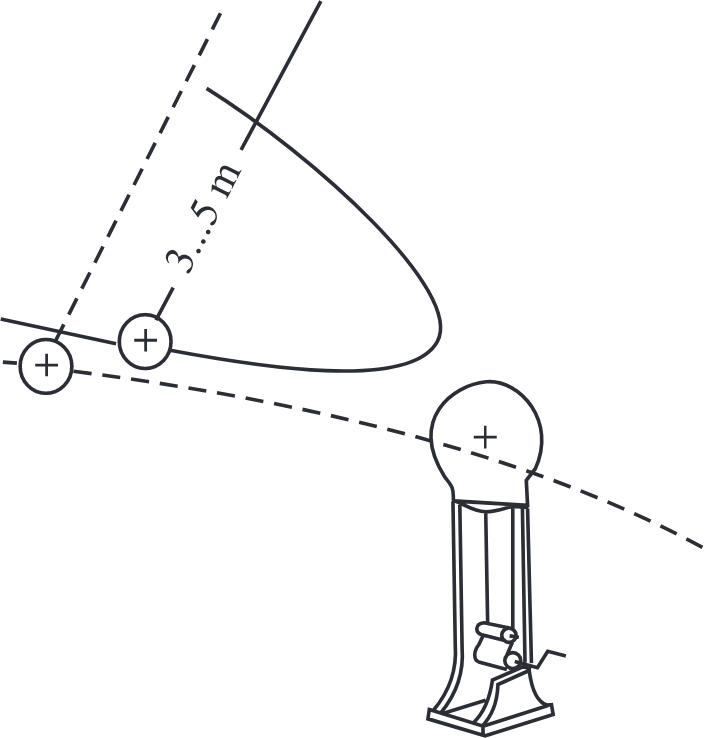
\includegraphics[width=0.4\textwidth]{fig/rutherford}
    \caption{Simularea experimentului}
\end{wrapfigure}

Se folosește un generator cu bandă, încărcat (Van de Graaf): o minge de
ping-pong se învelește în staniol (metalizare) și se suspendă de plafon cu un
fir de nailon de 3-5 m. În poziția de repaus, centrele celor două sfere (a
generatorului și a mingii) sunt pe aceeași direcție. Prin atingerea cu sfera
generatorului, mingea este încărcată și respinsă de acesta. Cu ajutorul unei
bare izolatoare, pendulul este îndepărtat de generator și aruncat apoi cu
viteză mare spre sau pe lângă acesta. Mingea va fi deviată, urmând o
traiectorie hiperbolică (fig. 2) sau, în cazul vitezelor
mici, eliptică ori circulară.

\clearpage

În urma experimentului, Rutherford a concluzionat că aproape întreaga masă a
atomului și sarcina sa pozitivă sunt concentrate într-un nucleu al atomului, cu
diametrul mai mic decât $10^{-14} - 10^{-15}$ m (diametrul atomului este
$10^{-9} - 10^{-10}$ m).

\begin{wrapfigure}{l}{0.45\textwidth}
    \centering
    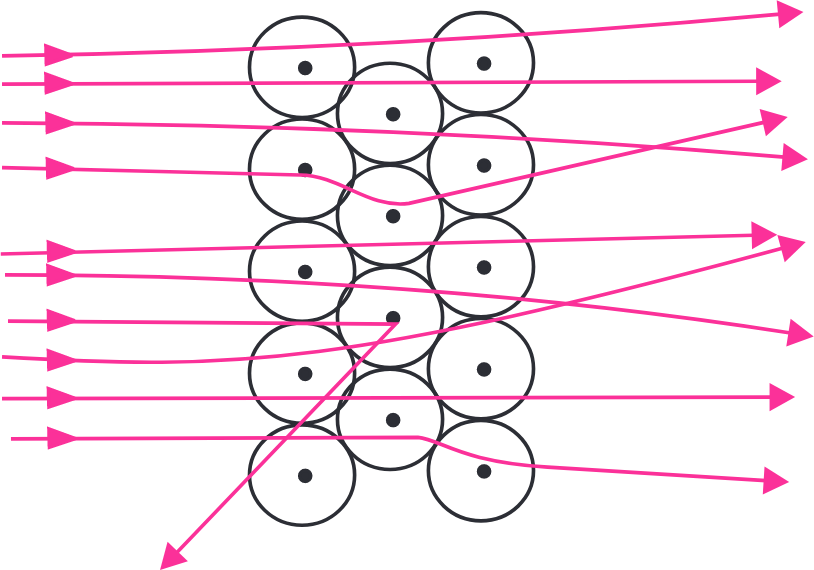
\includegraphics[width=0.4\textwidth]{fig/deviere}
    \caption{Devierea particulelor {\alpha} pe nucleele atomice ale unei foițe}
    \vspace{0.5cm}
    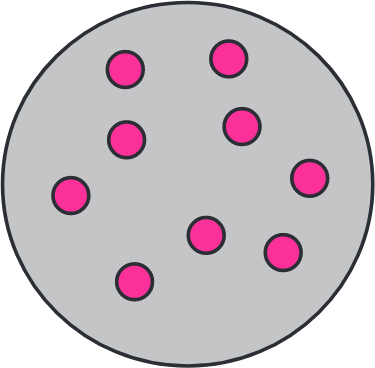
\includegraphics[width=0.15\textwidth]{fig/thomson}
    \captionsetup{width=5cm}
    \caption{Modelul lui Thompson („cozonac cu stafide”)}
\end{wrapfigure}

Prin urmare, cea mai mare parte a spațiului ocupat de un atom este lipsit de
substanță; altfel spus, atomul este mai mult „gol” decât „plin”. Particulele
{\alpha} pot trece pe lângă mii de nuclee fără a suferi devieri esențiale
(fig.3).

\emph{Modelul atomic} este un concept structural, constatat experimental. Se
cunosc \emph{modele atomice precuantice} (Thomson, Rutherford) și
\emph{modele atomice cuantice} (Bohr).

Modelul lui Thomson este un model static ce constă într-o sferă relativ mare,
cu sarcina pozitivă și raza de ordinul $10^{-10}$ m, în interiorul căreia sunt
dispuși electronii (fig. 4).

Acest model a fost infirmat de experimentul
Rutherford: dacă sarcina ar fi fost distribuită uniform în volumul atomului, un
număr mare de particule {\alpha} ar fi fost deviate. Modelul lui Thomson nu
poate explica structura de linii a spectrelor atomilor.

\clearpage

\subsection{Modelul planetar al atomului}

Modelul Rutherford aseamănă structura atomului cu sistemul solar. Masa și
sarcina pozitivă sunt concentrate într-un nucleu de dimensiuni mult mai mici
($10^{-15}$ m) decât ale atomului ($10^{-10}$ m). Electronii se rotesc în jurul
nucleului pe orbite circulare, forța de atracție dintre aceștia și nucleu fiind
de natură electrică.

Particulele subatomice sunt:
\begin{itemize}
    \item \emph{electronul}, încărcat negativ
    \item \emph{protonul}, încărcat pozitiv
    \item \emph{neutronul}, neutru
\end{itemize}

Modulul sarcinii negative a electronului este egal cu modulul sarcinii pozitive
a protonului. Particulele subatomice sunt așezate după aceeași regulă în toți
atomii: protonii și neutronii formează nucleul, cu sarcina pozitivă, în jurul
căruia se află electronii, la distanțe relativ mari, în număr egal cu protonii.
Atomul este deci neutru din punct de vedere electric.

Procesul prin care atomul pierde sau câștigă electroni se numește
\emph{ionizare}. Dacă atomul pierde unul sau mai mulți electroni, particula
rămasă se numește \emph{ion pozitiv}. Dacă atomul câștigă unul sau mai mulți
electroni, particula rămasă se numește \emph{ion negativ}.

Forțele de atracție electrostatice ce rețin electronii de nucleu acționează ca
forțe centripete.

\begin{wrapfigure}{r}{0.35\textwidth}
    \centering
    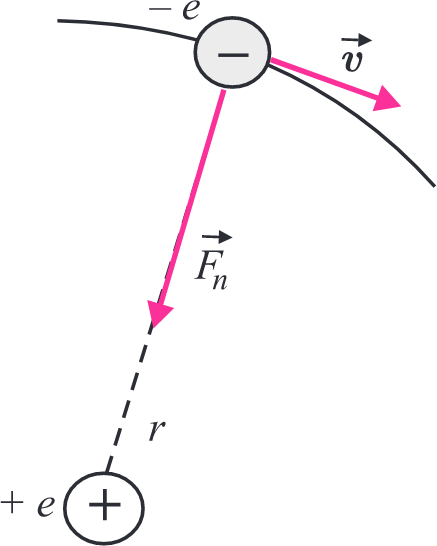
\includegraphics[width=0.3\textwidth]{fig/model_planetar}
    \caption{Mișcarea electronului în jurul nucleului}
\end{wrapfigure}

Conform modelului planetar, cel mai simplu sistem atomic este
\emph{atomul de hidrogen}, format dintr-un singur proton și un singur electron,
ce se mișcă în câmp coloumbian.

Considerând că electronul se mișcă pe o orbită circulară, energia sa totală
$E_t$ este suma energiei cinetice $E_c$ și energiei potențiale $E_p$:
\[ E_t = E_c + E_p \]

Aplicăm legea a II-a a lui Newton, \( F = ma \), unde forța care imprimă
electronului de masă $m$ accelerația centripetă \( \frac{v^2}{r} \) este forța
coulombiană \( F_c = \frac{1}{4\pi\varepsilon_0} \frac{e^2}{r^2} \):
\[ F_c = \frac{1}{4\pi\varepsilon_0} \frac{e^2}{r^2} = \frac{mv^2}{r} \]

Înmulțind relația cu \( \frac{r}{2} \), se obține energia cinetică a
electronului care se mișcă pe orbita circulară de rază $r$:
\[ E_c = \frac{mv^2}{2} = \frac{e^2}{8\pi\varepsilon_0 r} \]

Lucrul mecanic efectuat de $F_c$ pentru deplasarea electronului pe distanța
$r$:
\[
    L = F_c \cdot r = \frac{e^2}{4\pi\varepsilon_0 r^2} r
    = \frac{e^2}{4\pi\varepsilon_0 r} = - E_p
\]

Rezultă că \( E_p = - \frac{e^2}{4\pi\varepsilon_0 r} \) și deci:
\begin{equation}
    E_t = - \frac{e^2}{8\pi\varepsilon_0 r}
    \label{eq:1}
\end{equation}

Legile mecanicile clasicii sunt considerate valabile în acest model. Prin urmare, $E_t$ poate lua orice valoare între $-\infty$ și 0.

Se observă că \( E_p = -2E_c \) și \( E_t = -E_c = \frac{E_p}{2} \).

\subsubsection*{Deficiențele modelului planetar Rutherford}

Principala deficiență este cea a instabilității atomului. Un purtător de sarcină în
mișcare accelerată emite radiație, micșorând energia totală a electronului.
Raza sa va scădea, și eventual electronul va cădea pe nucleu. Experiența
confirmă însă stabilitatea în timp a atomilor.

Deoarece modelul Rutherford nu poate explica spectrele de emisie și absorbție
observate pe cale experimentală, s-a căutat un alt model, capabil să explice
aceste fenomene.
